\section{习题}

\subsection{时间复杂度与渐近符号}

\noindent1.给出渐近上界 $O$ 的定义,并证明
$3n^2+4n=O(n^2).$

\noindent\textbf{解答:}

\noindent\textbf{(1)$O$ 的定义:}
设 $f(n),g(n)$ 为非负函数。若存在常数 $c>0$ 与 $n_0$,使得对所有 $n\ge n_0$ 都有
$f(n)\le c\,g(n),$则称 $f(n)=O(g(n))$。

\noindent\textbf{(2)证明:}
令 $f(n)=3n^2+4n$,$g(n)=n^2$。当 $n\ge 1$ 时,有$4n \le 4n^2,$
因此
\[
3n^2+4n \le 3n^2+4n^2 = 7n^2.
\]
取 $c=7$,$n_0=1$,则对所有 $n\ge 1$ 都有
\[
3n^2+4n \le 7n^2 = c\,g(n).
\]
由渐近上界 $O$ 的定义可知
\[
3n^2+4n = O(n^2).
\]\\

\noindent2.给出算法符号渐近下界 $\Omega$ 的定义,并证明
$5n^2+2=\Omega\!\left(20n^{1.8}\right).$

\noindent\textbf{解答:}

\noindent\textbf{(1)$\Omega$ 的定义:}
设 $f(n),g(n)$ 为非负函数。若存在常数 $c>0$ 与 $n_0$,使得对所有 $n\ge n_0$ 都有
$f(n)\ge c\,g(n) \ge 0,$则称 $f(n)=\Omega(g(n))$。

\noindent\textbf{(2)证明:}
令 $f(n)=5n^2+2$,$g(n)=20n^{1.8}$。对 $n\ge 1$ 有
\[
5n^2+2 \ge 5n^2.
\]
取 $c=\frac14$,则需要验证当 $n\ge n_0$ 时
\[
5n^2 \ge \frac14 \cdot 20n^{1.8} = 5n^{1.8}.
\]
这等价于
\[
n^2 \ge n^{1.8}\quad \Longleftrightarrow\quad n^{0.2}\ge 1,
\]
对所有 $n\ge 1$ 成立。因此取 $n_0=1$,即可得到对所有 $n\ge 1$:
\[
5n^2+2 \ge \frac14\cdot 20n^{1.8}.
\]
所以
\[
5n^2+2=\Omega\!\left(20n^{1.8}\right).
\]\\

\noindent3.证明:
$0.12n^2\sqrt{n}+1000n^2\log n = O\!\left(n^{5/2}\right).$

\noindent\textbf{解答:}

\noindent\textbf{(1)$O$ 的定义:}
设 $f(n),g(n)$ 为非负函数。若存在常数 $c>0$ 与 $n_0$,使得对所有 $n\ge n_0$ 都有
$f(n)\le c\,g(n),$则称 $f(n)=O(g(n))$。

\noindent\textbf{(2)证明:}
令$
f(n)=0.12n^2\sqrt{n}+1000n^2\log n,\qquad g(n)=n^{5/2}.
$

当 $n\ge 1$ 时,
\[
0.12n^2\sqrt{n}=0.12n^{5/2}.
\]
又因为当 $n\ge 2$ 时有 $\log n \le \sqrt{n}$(例如令 $n=e^x$,则需证 $x\le e^{x/2}$,对 $x\ge \ln 2$ 成立),
所以对 $n\ge 2$:
\[
1000n^2\log n \le 1000n^2\sqrt{n}=1000n^{5/2}.
\]
因此当 $n\ge 2$ 时,
\[
f(n)=0.12n^{5/2}+1000n^2\log n \le (0.12+1000)n^{5/2}=1000.12\,n^{5/2}.
\]
取 $c=1000.12$,$n_0=2$,则对所有 $n\ge n_0$ 都有
\[
f(n)\le c\,g(n).
\]
由渐近上界 $O$ 的定义可知
\[
0.12n^2\sqrt{n}+1000n^2\log n = O\!\left(n^{5/2}\right).
\]\\

\noindent4.说明 $O(f(n))$ 的定义,并证明
$200n\log^3 n+102n^2\in O(n^2).$

\noindent\textbf{解答:}

\noindent\textbf{(1)$O$ 的定义:}
设 $f(n),g(n)$ 为非负函数。若存在常数 $c>0$ 与 $n_0$,使得对所有 $n\ge n_0$ 都有
$f(n)\le c\,g(n),$则称 $f(n)=O(g(n))$。

\noindent\textbf{(2)证明:}
令
\[
f(n)=200n\log^3 n+102n^2,\qquad g(n)=n^2.
\]
由于对任意常数 $a>0$ 都有 $\log n = o(n^a)$,取 $a=\frac13$,则存在 $n_0$ 使得当 $n\ge n_0$ 时
\[
\log n \le n^{1/3}\quad\Longrightarrow\quad \log^3 n \le n.
\]
于是当 $n\ge n_0$ 时,
\[
200n\log^3 n \le 200n\cdot n=200n^2.
\]
因此对所有 $n\ge n_0$,
\[
f(n)=200n\log^3 n+102n^2 \le 200n^2+102n^2=302n^2.
\]
取 $c=302$,即可得到当 $n\ge n_0$ 时 $f(n)\le c\,g(n)$。
由渐近上界 $O$ 的定义可知
\[
200n\log^3 n+102n^2\in O(n^2).
\]

\clearpage
\subsection{递归与分治}

\subsubsection{题型1:线性递推求解}

\noindent1.求解线性递归关系:
\[
\begin{cases}
X_{n+1}=\dfrac{9}{2}X_n-\dfrac{9}{2}X_{n-1},\quad n\ge 1,\\[6pt]
X_0=3,\ X_1=6.
\end{cases}
\]

\noindent\textbf{解答:}

该递归为二阶常系数齐次线性递推。设解形如 $X_n=r^n$,代入得特征方程
\[
r^{n+1}=\frac{9}{2}r^n-\frac{9}{2}r^{n-1}
\quad\Longrightarrow\quad
r^2-\frac{9}{2}r+\frac{9}{2}=0.
\]
解得
\[
r_1=3,\qquad r_2=\frac{3}{2}.
\]
故通解为
\[
X_n=A\cdot 3^n+B\cdot\left(\frac{3}{2}\right)^n.
\]
由初值 $X_0=3$ 得
\[
A+B=3.
\]
由初值 $X_1=6$ 得
\[
3A+\frac{3}{2}B=6.
\]
解得
\[
A=1\qquad B=2.
\]
因此递推式的显式解为
\[
\boxed{\,X_n=3^n+2\left(\frac{3}{2}\right)^n\, }.
\]

\noindent2.求解以下线性齐次递归方程:
\[
\begin{cases}
f(n)=f(n-1)+12f(n-2),\\
f(1)=1,\ f(0)=\dfrac12.
\end{cases}
\]

\noindent\textbf{解答:}

设解形如 $f(n)=r^n$,代入递推式得特征方程
\[
r^2=r+12 \quad\Longrightarrow\quad r^2-r-12=0.
\]
解得
\[
r_1=4,\qquad r_2=-3.
\]
故通解为
\[
f(n)=A\cdot4^n+B\cdot(-3)^n.
\]
由初值 $f(0)=\dfrac12$ 得
\[
A+B=\frac12.
\]
由初值 $f(1)=1$ 得
\[
4A-3B=1.
\]
联立解得
\[
A=\frac{5}{14},\qquad B=\frac17.
\]
因此递推式的显式解为
\[
\boxed{\,f(n)=\frac{5}{14}\cdot4^n+\frac17\cdot(-3)^n\, }.
\]

\subsubsection{题型2:排序问题}
\noindent{1.快速排序算法}

\begin{enumerate}
\item[(1)]说明快速排序算法的实现原理,并分析划分元素的选取对算法性能的影响;
\item[(2)]用 C/C++/Java 语言风格的伪代码描述快速排序算法实现过程;
\item[(3)]证明:在最好情况下,快速排序算法的时间复杂度为
$T(n)=O(n\log n)$;
\item[(4)]变式题:假定共有 $n=2^k$ 个元素,试分析该算法\textbf{最坏情况}下的时间复杂度。
\item[(5)]给定输入序列 $\{23,13,28,20,22,19,25\}$,将序列按照非递增顺序排列,
描述整个排序过程。假设在排序过程中,RandomizedPartition 过程总是选取序列中最后1个元素作为划分基准元素。 
\item[(6)]变式题:给定输入序列$\{13,3,18,10,12,9,15\},$
划分过程每次以\textbf{子序列第1个元素}作为划分基准,按\textbf{非递减序}排序。
\end{enumerate}

\noindent\textbf{解答:}

\noindent\textbf{(1)算法原理:}

快速排序是一种基于\textbf{分治策略}的排序算法。
假设排序序列为 $A[p\ldots r]$,
首先从序列中选取一个元素作为\textbf{划分基准},
将序列划分为三部分:
基准元素左侧元素均不大于基准,
右侧元素均不小于基准,
基准元素位于最终有序位置。
随后分别对左右子序列递归调用快速排序算法。

划分元素的选取直接影响算法效率。
若每次划分较为均匀,则递归深度为 $O(\log n)$;
若划分极不均匀,则算法性能退化。

\noindent\textbf{(2)算法伪代码:}

\begin{lstlisting}[language=C,style=codeStyle]
void QuickSort(Type a[], int p, int r)
{
    if (p < r)
    {
        int q = RandomizedPartition(a, p, r);
        QuickSort(a, p, q - 1);
        QuickSort(a, q + 1, r);
    }
}
\end{lstlisting}

\begin{lstlisting}[language=C,style=codeStyle]
int Partition(Type a[], int p, int r)
{
    int i = p, j = r;
    Type x = a[p];      // 基准元素

    while (true)
    {
        while (a[++i] < x && i < r);
        while (a[--j] > x);
        if (i >= j)
            break;
        Swap(a[i], a[j]);
    }
    a[p] = a[j];
    a[j] = x;
    return j;
}
\end{lstlisting}

\begin{lstlisting}[language=C,style=codeStyle]
int RandomizedPartition(Type a[], int p, int r)
{
    int i = Random(p, r);
    Swap(a[i], a[p]);
    return Partition(a, p, r);
}
\end{lstlisting}

\noindent\textbf{(3)最好情况下时间复杂度证明:}

在最好情况下,每次划分都将规模为 $n$ 的问题分成两个规模约为 $n/2$ 的子问题,
一次划分过程的时间复杂度为 $O(n)$,
故递归关系为
\[
T(n)=2T\left(\frac{n}{2}\right)+O(n).
\]
由主定理可得
\[
T(n)=O(n\log n).
\]

\noindent\textbf{(4)最坏情况时间复杂度分析:}

最坏情况发生在每次划分极不均匀(例如p总是当前子序列最小或最大元素),
从而把规模为 $n$ 的问题划分为规模分别为 $0$ 和 $n-1$ 的子问题。
一次划分需要线性时间 $cn$(扫描/交换),故递推式为
\[
T(n)=T(n-1)+T(0)+cn = T(n-1)+cn,\quad T(1)=\Theta(1).
\]
展开得
\[
T(n)=cn+c(n-1)+\cdots+c\cdot2+T(1)
= c\sum_{i=2}^{n} i + \Theta(1)
= \Theta(n^2).
\]
因此最坏情况下
\[
\boxed{T(n)=O(n^2)}.
\]
又因为题设 $n=2^k$,所以也可写为
\[
T(2^k)=O\big((2^k)^2\big)=O(4^k).
\]

\noindent\textbf{(5)排序过程:}

对序列 $\{23,13,28,20,22,19,25\}$ 的排序过程如下(注意为\textbf{非递增序}):
\[
\text{初始:}\ 23,\ 13,\ 28,\ 20,\ 22,\ 19,\ \underline{25}
\quad(\underline{25}\ \text{为基准元素})
\]
第一次划分(以 $25$ 为基准)后:
\[
28,\ \boxed{25},\ 23,\ 20,\ 22,\ 19,\ 13
\]
此时左子序列 $\{28\}$ 长度为 1,左子序列排序结束;处理右子序列
$\{23,20,22,19,13\}$,以最后一个元素为基准。
\[
28,\ \boxed{25},\ 23,\ 20,\ 22,\ 19,\ \underline{13}
\quad(\underline{13}\ \text{为基准元素})
\]
对右子序列继续划分(以 $13$ 为基准)后:
\[
28,\ \boxed{25},\ 23,\ 20,\ 22,\ \underline{19},\ \boxed{13}
\quad(\underline{19}\ \text{为基准元素})
\]
继续对子序列 $\{23,20,22,19\}$ 划分(以 $19$ 为基准)后:
\[
28,\ \boxed{25},\ 23,\ 20,\ 22,\ \boxed{19},\ \boxed{13}
\quad(\boxed{19}\ \text{就位})
\]
继续对子序列 $\{23,20,22\}$ 划分(以 $22$ 为基准)后:
\[
28,\ \boxed{25},\ 23,\ \boxed{22},\ 20,\ \boxed{19},\ \boxed{13}
\]
剩余待排序子序列 $\{23\}$ 和 $\{20\}$ 长度均为 1,排序结束。
最终结果为:
\[
\boxed{28,\ 25,\ 23,\ 22,\ 20,\ 19,\ 13}.
\]

\noindent\textbf{(6)排序过程:}

对序列 $\{13,3,18,10,12,9,15\}$ 的排序过程如下(注意为\textbf{非递减序}):
\[
\text{初始:}\ \underline{13},\ 3,\ 18,\ 10,\ 12,\ 9,\ 15
\quad(\underline{13}\ \text{为基准元素})
\]

第一次划分(以 $13$ 为基准)后:
\[
12,\ 3,\ 9,\ 10,\ \boxed{13},\ 18,\ 15
\]

此时左子序列 $\{12,3,9,10\}$,右子序列 $\{18,15\}$,
分别继续递归排序。

\[
\underline{12},\ 3,\ 9,\ 10,\ \boxed{13},\ 18,\ 15
\quad(\underline{12}\ \text{为基准元素})
\]

对左子序列划分(以 $12$ 为基准)后:
\[
10,\ 3,\ 9,\ \boxed{12},\ \boxed{13},\ 18,\ 15
\]

继续对子序列 $\{10,3,9\}$ 进行划分:
\[
\underline{10},\ 3,\ 9,\ \boxed{12},\ \boxed{13},\ 18,\ 15
\quad(\underline{10}\ \text{为基准元素})
\]

划分后:
\[
9,\ 3,\ \boxed{10},\ \boxed{12},\ \boxed{13},\ 18,\ 15
\]

继续对子序列 $\{9,3\}$ 进行划分:
\[
\underline{9},\ 3,\ \boxed{10},\ \boxed{12},\ \boxed{13},\ 18,\ 15
\quad(\underline{9}\ \text{为基准元素})
\]

划分后:
\[
3,\ \boxed{9},\ \boxed{10},\ \boxed{12},\ \boxed{13},\ 18,\ 15
\]

左子序列排序完成,继续对右子序列 $\{18,15\}$ 递归排序:
\[
3,\ \boxed{9},\ \boxed{10},\ \boxed{12},\ \boxed{13},\ \underline{18},\ 15
\quad(\underline{18}\ \text{为基准元素})
\]

划分后:
\[
3,\ \boxed{9},\ \boxed{10},\ \boxed{12},\ \boxed{13},\ 15,\ \boxed{18}
\]

剩余子序列长度均为 1,排序结束。
最终结果为:
\[
\boxed{3,\ 9,\ 10,\ 12,\ 13,\ 15,\ 18}.
\]

\noindent\textbf{2.两路归并(合并)排序算法}

\begin{enumerate}
\item[(1)]说明两路归并排序算法的原理;
\item[(2)]用类 C/C++/Python 语言伪代码写出上述算法的归并过程及归并排序过程;
\item[(3)]假定欲排序的元素个数为 $2^n$,对该算法最好情况下的时间复杂度(比较次数)进行分析。
\end{enumerate}

\noindent\textbf{解答:}

\noindent\textbf{(1)两路归并排序原理:}两路归并排序是一种基于\textbf{分治策略}的稳定排序算法。其思想是:
将待排序序列不断二分为两个子序列,直到每个子序列长度为 $1$(天然有序),
然后在回溯阶段将两个已排序的子序列通过\textbf{归并(merge)}操作合并成一个更长的有序序列,
最终得到整体有序结果。归并时使用两个指针分别扫描两段有序序列,
每次取较小(非递减排序)者放入辅助数组,直至合并完成。

\noindent\textbf{(2)类 C/C++/Python 伪代码:}

\begin{lstlisting}[language=C,style=codeStyle]
void mergeSort(Type a[], int left, int right)
{
    if (left < right) {
        int i = (left + right) / 2;
        mergeSort(a, left, i);
        mergeSort(a, i + 1, right);
        merge(a, b, left, i, right);
        copy(a, b, left, right);
    }
}
\end{lstlisting}

\begin{lstlisting}[language=C,style=codeStyle]
void merge(Type a[], Type d[], int l, int m, int r)
{
    int i = l, j = m + 1, k = l;
    while (i <= m && j <= r) {
        if (a[i] <= a[j])
            d[k++] = a[i++];
        else
            d[k++] = a[j++];
    }
    if (i > m)
        for (int q = j; q <= r; q++)
            d[k++] = a[q];
    else
        for (int q = i; q <= m; q++)
            d[k++] = a[q];
}
\end{lstlisting}

\noindent\textbf{(3)最好情况下时间复杂度(比较次数)分析:}

两路归并排序不断将序列二分,直到每个子序列只剩一个元素为止,然后自底向上进行归并。
设待排序序列长度为$N=2^n,$则递归(划分)深度为 $n$ 层,因为每次划分都将序列分为两部分。

在归并阶段,每一层都需要对所有元素进行合并比较。
最好情况下,每次比较都能确定一个元素的位置,因此在一层合并中,
若该层需要合并的元素总数为 $2^n$,则该层最多只需比较$2^n-1$
次即可完成合并(最后一个元素无需比较即可确定)。

因此共有 $n$ 层归并,每层比较次数为 $2^n-1$,最好情况下总比较次数为
$T(2^n)=n(2^n-1).$
于是$T(2^n)=O(n2^n).$
又由于 $N=2^n \Rightarrow n=\log_2 N$,因此$T(N)=O(N\log N).$


\noindent\textbf{3.用分治法设计一个算法,找出一个数组中的最大的三个数,写出算法 C 语言的实现。
假定共有 $n=2^m$ 个元素,分析算法的复杂度。}

\noindent\textbf{解答:}

\noindent\textbf{(1)算法思想:}

把区间 $[l,r]$ 二分为 $[l,mid]$ 与 $[mid+1,r]$,分别递归求出左右区间的前三大元素;
再将左右区间得到的 6 个候选数合并,取其中最大的 3 个作为当前区间的前三大。
当区间长度为 1 时,前三大为该元素本身,其余用一个极小值(如 $-\infty$)填充。

\noindent\textbf{(2)C 语言实现:}

\begin{lstlisting}[language=C,style=codeStyle]
#include <limits.h>
/* 把 v 插入到 (x1 >= x2 >= x3) 中,保持前三大 */
void insert3(int v, int *x1, int *x2, int *x3)
{
    if (v > *x1) {
        *x3 = *x2;
        *x2 = *x1;
        *x1 = v;
    } else if (v > *x2) {
        *x3 = *x2;
        *x2 = v;
    } else if (v > *x3) {
        *x3 = v;
    }
}
/* 分治求 A[l..r] 中最大的三个数,结果放到 *m1,*m2,*m3 中 */
void max3(int A[], int l, int r, int *m1, int *m2, int *m3)
{
    if (l == r) {
        *m1 = A[l];
        *m2 = INT_MIN;
        *m3 = INT_MIN;
        return;
    }
    int mid = (l + r) / 2;
    int L1, L2, L3, R1, R2, R3;
    max3(A, l, mid, &L1, &L2, &L3);
    max3(A, mid + 1, r, &R1, &R2, &R3);
/* 合并:从 6 个候选中选最大三个 */
    *m1 = INT_MIN; *m2 = INT_MIN; *m3 = INT_MIN;
    insert3(L1, m1, m2, m3);
    insert3(L2, m1, m2, m3);
    insert3(L3, m1, m2, m3);
    insert3(R1, m1, m2, m3);
    insert3(R2, m1, m2, m3);
    insert3(R3, m1, m2, m3);
}

/* 调用示例:
   int m1, m2, m3;
   max3(A, 0, n-1, &m1, &m2, &m3);
*/
\end{lstlisting}

\noindent\textbf{(3)时间复杂度分析:}

设 $T(n)$ 为在 $n$ 个元素中找最大三个数的时间。
当 $n=1$ 时,$T(1)=\Theta(1)$;
当 $n>1$ 时,递归求解两个规模为 $n/2$ 的子问题,
合并阶段只需在 6 个候选数中选出最大 3 个,为常数时间 $\Theta(1)$。
因此递推式为
\[
T(n)=2T\left(\frac{n}{2}\right)+\Theta(1).
\]
题设 $n=2^m$,递归深度为 $m=\log_2 n$,递归树共有 $n$ 个叶子结点,
内部结点数为 $n-1$,每个内部结点合并代价为常数,
故
\[
T(n)=\Theta(n).
\]
因此算法时间复杂度为
\[
\boxed{T(n)=O(n)}.
\]

\clearpage
\subsection{动态规划}

\noindent\textbf{1. 最长公共子序列问题:}给定两个序列 $X=\langle x_1,x_2,\dots,x_m\rangle$ 和 $Y=\langle y_1,y_2,\dots,y_n\rangle$,
求它们的最长公共子序列(LCS)。
例如 $X=\langle A,B,C,B,D\rangle$,
$Y=\langle B,D,C,A,B,A\rangle$,
则最长公共子序列为 $Z=\langle B,C,B,A\rangle$。
试用动态规划方法求解最长公共子序列问题,要求:

(1) 写出递归关系式;

(2) 基于 C/C++ 伪代码描述算法流程,输出包括 LCS 长度与 LCS 序列;

(3) 分析时间复杂度;

(4) 利用 LCS 求解最长递减子序列(LIS),给出算法与伪代码。

\noindent\textbf{解答:}

\noindent\textbf{(1) 递归关系式:}
令 $c[i][j]$ 表示序列 $X[1..i]$ 与 $Y[1..j]$ 的最长公共子序列长度,则边界为
$$
c[i][0]=0,\quad 1\le i\le m;\qquad c[0][j]=0,\quad 1\le j\le n.
$$

为恢复一个最长公共子序列,常用辅助数组 $b[i][j]$ 记录转移方向:
当 $x_i=y_j$ 时记录来自左上;否则记录来自上或左(取较大者)。

$$
c[i][j]=
\begin{cases}
0, & i=0, j=0 \\[6pt]
c[i-1][j-1]+1, & i,j>0;\ x_i = y_j \\[6pt]
\max\{c[i][j-1],\ c[i-1][j]\}, & i,j>0;\ x_i \neq y_j
\end{cases}
$$


\noindent\textbf{(2) 代码:}
\begin{lstlisting}[language=C,style=codeStyle]
void LCSLength(int m, int n, char *x, char *y, int **c, int **b)
{
    int i, j;
    // 初始化边界:任意序列与空序列的LCS长度为0
    for (i = 0; i <= m; i++) c[i][0] = 0;
    for (j = 0; j <= n; j++) c[0][j] = 0;
    // 动态规划填表:从小规模子问题推到大规模子问题
    for (i = 1; i <= m; i++) {
        for (j = 1; j <= n; j++) {
            if (x[i] == y[j]) {              // xi == yj
                c[i][j] = c[i-1][j-1] + 1;
                b[i][j] = 1;                 // 记录来自左上
            } else if (c[i-1][j] >= c[i][j-1]) {
                c[i][j] = c[i-1][j];
                b[i][j] = 2;                 // 记录来自上
            } else {
                c[i][j] = c[i][j-1];
                b[i][j] = 3;                 // 记录来自左
            }
        }
    }
}
void LCS(int i, int j, char *x, int **b)
{
    if (i == 0 || j == 0) return;     // 回溯到边界,结束
    if (b[i][j] == 1) {               // 来自左上:说明匹配到一个字符
        LCS(i-1, j-1, x, b);
        printf("%c", x[i]);           // 输出该字符(属于LCS)
    } else if (b[i][j] == 2) {        // 来自上:丢弃 xi
        LCS(i-1, j, x, b);
    } else {                          // 来自左:丢弃 yj
        LCS(i, j-1, x, b);
    }
}
\end{lstlisting}

\noindent\textbf{(3) 复杂度:}
表格大小为 $m\times n$,每个格子 $O(1)$ 计算,
所以时间复杂度为 $O(mn),$
空间复杂度为 $O(mn).$
回溯输出最多走 $m+n$ 步,为 $O(m+n).$

\noindent\textbf{(4)利用最长公共子序列求解最长递减子序列}

由于最长递减子序列问题是求解一个给定序列的最长递减子序列,
可以将其转化为最长公共子序列问题来求解。
其基本思想是:  
对原序列进行排序,得到其\textbf{降序排列}后的新序列,
再对原序列与该降序序列求最长公共子序列,
则该最长公共子序列即为原序列的一个最长递减子序列。
显然,只要将原序列降序排列,
原序列与降序序列的最长公共子序列就对应于原序列的最长递减子序列。
需要注意的是,在最长公共子序列算法中,
两个参数数组通常是字符数组;
而在求解最长递减子序列问题时,
应先将这两个参数数组改为\textbf{整型数组}。

\noindent\textbf{算法步骤如下:}

\begin{lstlisting}[language=C,style=codeStyle]
void LIS(int a[], int x[], int m)
{
    // 该算法求解 x[1..m] 这个长度为 m 的整型数组的最长递减子序列长度
    for (int i = 1; i <= m; i++)       // 输入数组 x
        scanf("%d", &x[i]);
    for (int i = 1; i <= m; i++)       // 数组 a 为数组 x 的副本
        a[i] = x[i];
    mergesort(a, 1, m);                // 对数组 a 进行降序排序
    LCSLength(x, a, m, m);              // 求数组 x 与数组 a 的最长公共子序列长度
}
\end{lstlisting}

\noindent\textbf{2. 0/1 背包问题:}
给定 $n$ 个物品和一个背包,物品 $i$ 的重量为 $w_i$,
价值为 $v_i$,背包容量为 $C$。
适当选择装入背包的物品以使装入物品的总价值最大。
试用动态规划法求解 0/1 背包问题,要求:

\begin{enumerate}
  \item[(1)]写出 0/1 背包问题最优解的递归方程式;
  \item[(2)]用类 C/C++/Python 语言伪代码描述算法流程,算法输出结果为装入物品和最大价值;
  \item[(3)]分析上面所描述算法的时间复杂度。
\end{enumerate}

\noindent\textbf{解答:}

\noindent\textbf{(1)递归方程式:}
定义状态 $m(i,j)$ 表示只考虑物品 $i,i+1,\dots,n$,
且背包容量为 $j$($0\le j\le C$)时的最大总价值,则有
$$
m(i,j)=
\begin{cases}
\max\{m(i+1,j),\ m(i+1,j-w_i)+v_i\}, & j\ge w_i,\\
m(i+1,j), & 0\le j<w_i.
\end{cases}
$$
边界条件为
$$
m(n,j)=
\begin{cases}
v_n, & j\ge w_n,\\
0, & 0\le j<w_n.
\end{cases}
$$

\noindent\textbf{(2)算法伪代码:}

\begin{lstlisting}[language=C,style=codeStyle]
void knapsack(Type v[], int w[], int c, int n, Type **m)
{
    int jMax = min(w[n] - 1, c);
    for (int j = 0; j <= jMax; j++)
        m[n][j] = 0;
    for (int j = w[n]; j <= c; j++)
        m[n][j] = v[n];
    for (int i = n - 1; i > 1; i--) {
        jMax = min(w[i] - 1, c);
        for (int j = 0; j <= jMax; j++)
            m[i][j] = m[i+1][j];
        for (int j = w[i]; j <= c; j++)
            m[i][j] = max(m[i+1][j], m[i+1][j - w[i]] + v[i]);
    }
    m[1][c] = m[2][c];
    if (c >= w[1])
        m[1][c] = max(m[1][c], m[2][c - w[1]] + v[1]);
}
\end{lstlisting}

\noindent\textbf{(3)时间复杂度:}
状态表规模约为 $n\times c$,
每个状态转移为 $O(1)$,
因此时间复杂度为$O(nc),$
空间复杂度为存储二维数组 $m$ 的$O(nc).$

\noindent\textbf{3.最大子段和问题:}
给定由 $n$ 个整数(也可能为负整数)组成的整数序列
$
a_1,a_2,\dots,a_n,
$
求该序列中子段
$
\sum_{k=i}^{j} a_k (1\le i\le j\le n)
$
的最大值。
当所有整数均为负整数时,规定最大子段和为 $0$。
根据上述描述,最大子段和定义为
$
\max\left\{\,0,\ \max_{1\le i\le j\le n}\sum_{k=i}^{j} a_k \right\}.
$

\noindent\textbf{(1)递推式/状态方程}

\noindent
令
$
b[j]
$
表示\textbf{以元素 $a[j]$ 结尾的最大子段和},则有递推关系:
$$
b[j] = \max\{\, b[j-1] + a[j],\ a[j] \}, 1\le j\le n,
$$
其中 $b[0]=0$。
整个序列的最大子段和为
$
\max_{1\le j\le n} b[j],
$
若该最大值为负,则结果取 $0$。

\noindent\textbf{(2)算法伪代码与复杂度分析}

\begin{lstlisting}[language=C,style=codeStyle]
int MaxSum(int n, int *a)
{
    int sum = 0;
    int b = 0;
    for (int i = 1; i <= n; i++) {
        if (b > 0) b = b + a[i];
        else b = a[i];
        if (sum < b) sum = b;
    }
    return sum;
}
\end{lstlisting}

\noindent\textbf{时间复杂度分析:}
算法只对序列进行一次线性扫描,
每次循环中的操作均为常数时间,
因此时间复杂度为
$
O(n).
$
算法仅使用常数个辅助变量,空间复杂度为
$
O(1).
$

\noindent\textbf{(3)求第一个取得最大子段和的子段起止位置}

\noindent
在上述算法基础上,通过增加下标变量即可确定第一个取得最大子段和的子段位置。

\begin{lstlisting}[language=C,style=codeStyle]
void MaxSumPos(int n, int *a, int &sum, int &l, int &r)
{
    int sum = 0;     // 全局最大
    int b = 0;       // 以当前位置结尾的最大子段和
    int start = 1;   // 当前子段的起点候选
    l = 0; r = 0;  // 若最大和为0,可按需要返回(0,0)
    for (int i = 1; i <= n; i++) {
        if (b > 0) {
            b = b + a[i];
        } else {
            b = a[i];
            start = i;     // 重新开始子段
        }
        if (sum < b) {
            sum = b;
            l = start;
            r = i;
        }
    }
}
\end{lstlisting}

\noindent\textbf{说明:}
当存在多个子段取得相同的最大子段和时,
上述算法由于只在 \texttt{b > sum} 时更新结果,
因此得到的是\textbf{第一个}取得最大子段和的子段,
其起始位置为 $l$,结束位置为 $r$。

\noindent\textbf{4. 答题顺序的期望奖励最大化:}
在一次测试中有 $N$ 道题目,受试者可以自行决定答题顺序。
如果第 $i$ 道题回答正确(正确概率为 $p_i$),则可获得 $R_i$ 分;
如果回答错误,则测试立即终止。
请确定一种合适的答题顺序,使受试者获得奖励的\textbf{期望分数最大化}。

\noindent\textbf{解答:}

\noindent\textbf{(1)动态规划递归式:}
\noindent 设 $S\subseteq\{1,2,\dots,N\}$ 表示\textbf{当前还未作答}的题目集合。
令 $F(S)$ 表示:在\textbf{尚未答错终止}的前提下,只作答集合 $S$ 中题目所能获得的\textbf{最大期望得分}。

\noindent 边界条件:
$
F(\varnothing)=0.
$

\noindent 若选择下一题做 $i\in S$,则:
答对(概率 $p_i$)得到 $R_i$ 分并继续做 $S\setminus\{i\}$;
答错(概率 $1-p_i$)测试终止,后续得分为 $0$。
因此递推为
$$
F(S)=\max_{i\in S}\Bigl(p_i\bigl(R_i+F(S\setminus\{i\})\bigr)\Bigr).
$$

\noindent\textbf{(2)由递推式得到最优排序规则:}

考虑仅比较两道题 $i$ 与 $j$ 的先后次序。
设做完它们之后其余题目带来的最优期望为同一个常数 $X$(来自 $F(\cdot)$ 的最优后缀值)。

若顺序为 $i\to j$,期望为
$
E_{i\to j}=p_i\Bigl(R_i+p_j(R_j+X)\Bigr).
$
若顺序为 $j\to i$,期望为
$
E_{j\to i}=p_j\Bigl(R_j+p_i(R_i+X)\Bigr).
$

令 $E_{i\to j}\ge E_{j\to i}$,展开并约去含 $X$ 的相同项,可得等价条件:
$
p_iR_i(1-p_j)\ \ge\ p_jR_j(1-p_i).
$

当 $p_i<1,\ p_j<1$ 时,两边同除以 $(1-p_i)(1-p_j)>0$ 得到排序准则:
$
\frac{p_iR_i}{1-p_i}\ \ge\ \frac{p_jR_j}{1-p_j}.
$

因此最优答题策略为:计算每题的关键值
$
K_i=\frac{p_iR_i}{1-p_i},
$
并按 $K_i$ \textbf{从大到小排序}后依次作答。
若 $p_i=1$,则 $1-p_i=0$,可视为 $K_i=+\infty$,应排在最前面。

\noindent\textbf{(3)算法伪代码:}

\begin{lstlisting}[language=C,style=codeStyle]
typedef struct {
    double p;     // 正确概率 p_i
    double R;     // 得分 R_i
    int id;       // 题号
    double key;   // K_i = p_i*R_i/(1-p_i)
} Item;

double MaxExpectedScore(int N, Item A[])
{
    // 计算 key
    for (int i = 1; i <= N; i++) {
        if (A[i].p >= 1.0) A[i].key = 1e100;     // 视为 +infty
        else A[i].key = A[i].p * A[i].R / (1.0 - A[i].p);
    }
    // 按 key 从大到小排序(可用快排/归并等)
    SortByKeyDesc(A, N);
    // 按该顺序计算最大期望得分
    double ans = 0.0;
    double survive = 1.0;  // 目前尚未终止的概率
    for (int i = 1; i <= N; i++) {
        ans += survive * A[i].p * A[i].R;
        survive *= A[i].p;
    }
    return ans;
}
\end{lstlisting}

\noindent\textbf{(4)复杂度分析:}计算 $N$ 个关键值需要 $O(N)$ 时间;
排序需要 $O(N\log N)$ 时间;
最后线性扫描计算期望需要 $O(N)$ 时间。
因此总时间复杂度为
$
O(N\log N).
$
除排序所需的额外空间外,算法仅使用常数个辅助变量,额外空间为 $O(1)$(不计排序实现)。

\clearpage
\subsection{贪心算法}

\noindent\textbf{1. 活动安排:}考虑利用贪心算法求解。

(1)用类 C/C++/Python 伪代码描述算法求解步骤,并分析算法复杂度;

(2)说明算法采用的贪心策略;

(3)给出问题具有最优子结构性质的定义,证明活动安排问题具有最优子结构性质;

(4)针对下述活动集合,给出一个参加活动个数最多的安排。
\[
\begin{array}{c|cccccccc}
\hline
\text{活动 } i & 1 & 2 & 3 & 4 & 5 & 6 & 7 & 8\\
\hline
\text{起始时间 } s[i] & 1 & 2 & 3 & 4 & 5 & 6 & 7 & 8\\
\text{结束时间 } f[i] & 6 & 4 & 5 & 10 & 8 & 9 & 11 & 13\\
\hline
\end{array}
\]

\noindent\textbf{解答:}

\noindent\textbf{(1)代码与复杂度:}

\begin{lstlisting}[language=C,style=codeStyle]
void GreedySelector(int n, int s[], int f[], bool A[])
{
    A[1] = true;          // 选择第一个活动
    int j = 1;
    for (int i = 2; i <= n; i++) {
        if (s[i] >= f[j]) {
            A[i] = true; // 选择活动 i
            j = i;
        } else {
            A[i] = false;
        }
    }
}
\end{lstlisting}

\noindent\textbf{算法复杂度分析:}
排序耗时为 $O(n\log n)$,选择过程为一次线性扫描,耗时为 $O(n)$。
因此总时间复杂度为
$T(n)=O(n\log n)+O(n)=O(n\log n).$
额外空间复杂度(除输入外)为 $O(1)$。

\noindent\textbf{(2)说明算法采用的贪心策略;}
\textbf{按活动的结束时间从小到大排序},每次选择\textbf{当前结束时间最早且与已选活动不冲突的活动}。
该策略能够为后续活动留下尽可能多的时间,从而得到参加活动个数最多的安排。

\noindent\textbf{(3)最优子结构性质}

\noindent\textbf{最优子结构性质的定义:}
若一个问题的最优解包含其子问题的最优解,则称该问题具有最优子结构性质。

\noindent\textbf{证明活动安排问题具有最优子结构性质:}
设在某一最优安排中,首先选择的活动为 $A_k$。
由于活动互不冲突,后续可选活动必须满足开始时间不早于 $A_k$ 的结束时间 $f_k$。
因此,在选择 $A_k$ 之后,剩余问题转化为在集合
$\{A_i \mid s_i \ge f_k\}$
中选择最多个互不冲突活动的子问题,该子问题仍然是活动安排问题。
若该子问题未取最优解,则可用更优的子问题解替换,从而得到更多活动,与原最优性矛盾。
故活动安排问题具有最优子结构性质。

\noindent\textbf{(4)针对下述活动集合,给出一个参加活动个数最多的安排。}

先按结束时间 $f[i]$ 从小到大排序(括号内为 $(s[i],f[i])$):
$$A_2(2,4),\ A_3(3,5),\ A_1(1,6),\ A_5(5,8),\ A_6(6,9),\ A_4(4,10),\ A_7(7,11),\ A_8(8,13).$$

按贪心策略选择:$
A_2(2,4)\ \rightarrow\ A_5(5,8)\ \rightarrow\ A_8(8,13).$

因此,一个参加活动个数最多的安排为:
$\boxed{\{A_2,\ A_5,\ A_8\}}$最多可参加的活动个数为:$\boxed{3}.$

\noindent\textbf{2. 背包问题:}
给定 $n$ 种物品和 1 个背包,其中物品 $i$ 的重量是 $w_i$,
其价值为 $v_i$,背包的容量为 $C$。
在选择物品 $i$ 装入背包时,可以选择物品 $i$ 的一部分,
请问应如何选择装入背包的物品,使得装入背包中物品的总价值最大?
\begin{enumerate}
  \item [(1)]给出此优化问题的整数规划数学公式,即问题的形式化描述。
  \item [(2)]给出该问题贪心算法求解的贪心策略。
  \item [(3)]基于 C/C++/Java/Python 等高级编程语言写出贪心算法的伪代码。
  \item [(4)]分析(3)中给出的贪心算法的时间复杂性。
  \item [(5)]给定 4 种物品重量分别为 $\{10,40,55,20\}$,价值分别为 $\{20,120,55,100\}$,背包容量是 $100$,求背包的最大价值以及对应的放入背包的物品重量。
\end{enumerate}

\noindent\textbf{解答:}

\noindent\textbf{(1)整数规划数学公式:}
设决策变量 $x_i$ 表示物品 $i$ 放入背包的比例。
由于题目说明“可以选择物品 $i$ 的一部分”,因此$
0 \le x_i \le 1,\quad i=1,2,\dots,n.$
目标是在容量约束下最大化总价值:
$\max \sum_{i=1}^{n} v_i x_i$
约束为:
$\sum_{i=1}^{n} w_i x_i \le C,0 \le x_i \le 1\ (i=1,2,\dots,n).$

\noindent\textbf{(2)贪心策略:}
令单位重量价值(价值密度)为$r_i=\frac{v_i}{w_i}.$
贪心策略为\textbf{按 $r_i=\dfrac{v_i}{w_i}$ 从大到小排序},
优先选择价值密度最高的物品尽可能多地装入背包;
若剩余容量不足以装下当前物品,则装入该物品的相应比例直至背包恰好装满。

\noindent\textbf{(3)贪心算法伪代码}

\begin{lstlisting}[language=C,style=codeStyle] 
void Knapsack(int n, float M, float v[], float w[], float x[])
{
    Sort(n, v, w);    // 按 v[i]/w[i] 从大到小排序
    for (int i = 1; i <= n; i++)
    x[i] = 0;
    float c = M;
    int i;
    for (i = 1; i <= n; i++) {
        if (w[i] > c) break;   // 剩余容量不足,无法装入整个物品 i
        x[i] = 1;              // 装入整个物品 i
        c -= w[i];
    }
    if (i <= n) x[i] = c / w[i];   // 装入物品 i 的一部分
}
\end{lstlisting}

\noindent\textbf{(4)时间复杂性分析:}主要开销来自排序:按 $\frac{v_i}{w_i}$ 排序需要 $O(n\log n)$;
排序后的一次线性扫描装包为 $O(n)$。
因此总时间复杂度为$
T(n)=O(n\log n).$
额外空间复杂度:若采用原地排序并用数组 $x$ 存放结果,则为 $O(n)$(存储 $x$),
除输出外的辅助空间可视具体排序实现而定。

\noindent\textbf{(5)计算最大价值及对应放入物品重量}

给定 $4$ 种物品:$
w=\{10,40,55,20\},v=\{20,120,55,100\},C=100.$

先计算价值密度:
$\frac{v_1}{w_1}=2,
\frac{v_2}{w_2}=3,
\frac{v_3}{w_3}=1,
\frac{v_4}{w_4}=5.$

按 $\frac{v_i}{w_i}$ 从大到小排序的顺序为:$A_4,\ A_2,\ A_1,\ A_3.$

按贪心装入:
\begin{itemize}
  \item 先装入 $A_4$($w_4=20$),剩余容量 $100-20=80$,获得价值 $100$;
  \item 再装入 $A_2$($w_2=40$),剩余容量 $80-40=40$,累计价值 $100+120=220$;
  \item 再装入 $A_1$($w_1=10$),剩余容量 $40-10=30$,累计价值 $220+20=240$;
  \item 最后装入 $A_3$ 的一部分:$\dfrac{30}{55}$,
        得到价值 $55\cdot\dfrac{30}{55}=30$,背包恰好装满。
\end{itemize}

因此最大价值为:$V_{\max}=100+120+20+30=\boxed{270}.$

对应放入背包的物品重量为:$w_4=20, w_2=40, w_1=10, w_3\cdot\frac{30}{55}=30,$

总重量为:$20+40+10+30=\boxed{100}.$

\noindent\textbf{3.哈夫曼编码:}
哈夫曼编码是用于数据文件压缩的编码方法,
给出出现频率高的字符较短的编码,
出现频率较低的字符以较长的编码,
可以大大缩短总码长。
对每一个字符规定一个 0、1 串作为其代码,
要求任一字符的代码都不是其他字符代码的前缀的编码方案称为前缀码。
使平均码长达到最小的前缀码编码方案称为哈夫曼编码。
给定编码字符集 $M$,
$M$ 中字符 $m$ 的出现频率分布为 $f(m)$。

\begin{enumerate}
  \item [(1)]详细说明构造哈夫曼编码树的贪心过程。
  \item [(2)]假定有字符 $a,b,c,d$,
        出现频率为 $f(a)=15,\ f(b)=25,\ f(c)=45,\ f(d)=60$,
        画出哈夫曼编码树;
  \item [(3)]给出哈夫曼编码的计算复杂度(假设共有 $n$ 个字符);
  \item [(4)]假设 $x$ 和 $y$ 是 $M$ 中具有最小频率的两个字符。
        证明:存在 $M$ 的哈夫曼编码使 $x$ 和 $y$ 具有相同码长且仅最后一位编码不同。
\end{enumerate}

\noindent\textbf{解答:}

\noindent\textbf{(1)详细说明构造哈夫曼编码树的贪心过程。}

设字符集为 $M$,每个字符 $m\in M$ 的出现频率为 $f(m)$。
构造哈夫曼编码树的贪心过程如下:

\begin{enumerate}
  \item [(i)]将每个字符 $m$ 看成一棵只有一个结点的二叉树(叶子结点),其权值为 $f(m)$。
  \item [(ii)]在所有当前树(或结点)中,\textbf{反复选择权值最小的两棵树} $T_1,T_2$(贪心选择)。
  \item [(iii)]新建一个父结点,将 $T_1,T_2$ 分别作为其左、右子树,
        父结点权值取为两子树权值之和:$w(\text{parent}) = w(T_1)+w(T_2).$
  \item [(iv)]用这棵新树替代原来的两棵树,继续步骤 2,直到只剩下一棵树为止,
        该树即为哈夫曼编码树。
  \item [(v)]规定从根到叶子的边上左分支记为 $0$、右分支记为 $1$(或反之也可),
        则每个字符的编码就是其叶子结点对应的根路径上的 0/1 串。
\end{enumerate}

该算法的贪心选择是“每次合并当前\textbf{最小权值的两棵树}”,
它保证了最终得到的前缀码具有最小的加权路径长度(最小平均码长)。

\noindent\textbf{(2)画出哈夫曼编码树。}

已知:$f(a)=15,f(b)=25,f(c)=45,f(d)=60.$
按贪心步骤合并:$15+25=40,40+45=85,85+60=145.$
因此可得到如下哈夫曼树(左边标 0、右边标 1;左右互换也同样正确):

\begin{center}
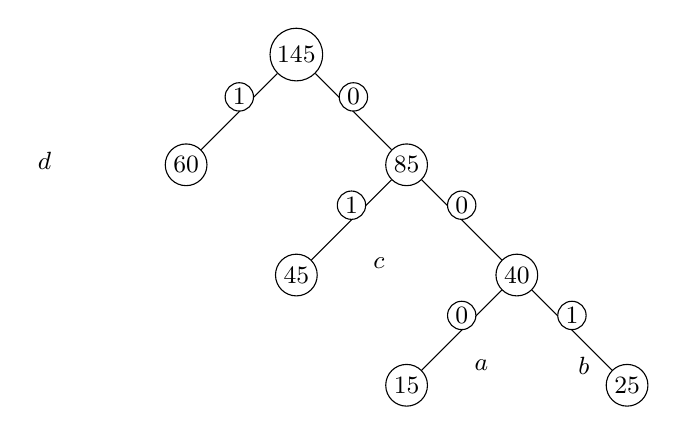
\begin{tikzpicture}[
  level distance=14mm,
  sibling distance=28mm,
  every node/.style={draw, circle, inner sep=1.5pt, font=\small},
  edge from parent/.style={draw,-},
  lab/.style={midway, fill=white, inner sep=1pt, font=\small}
]
\node {145}
  child { node {60}
    child[missing]
    child[missing]
  edge from parent node[lab, above] {1}
  }
  child { node {85}
    child { node {45}
      child[missing]
      child[missing]
      edge from parent node[lab, above] {1}
    }
    child { node {40}
      child { node {15}
        child[missing]
        child[missing]
        edge from parent node[lab, above] {0}
      }
      child { node {25}
        child[missing]
        child[missing]
        edge from parent node[lab, above] {1}
      }
      edge from parent node[lab, above] {0}
    }
    edge from parent node[lab, above] {0}
  };

% 给叶子加标签(把频率对应到字符)
\node[draw=none, font=\small] at (-3.2,-1.35) {$d$};
\node[draw=none, font=\small] at (1.05,-2.65) {$c$};
\node[draw=none, font=\small] at (2.35,-3.95) {$a$};
\node[draw=none, font=\small] at (3.65,-3.95) {$b$};
\end{tikzpicture}
\end{center}

由上图(取左边为 0、右边为 1)可给出一组编码:
$d:1,c:01,a:000,b:001.$

\noindent\textbf{(3)给出哈夫曼编码的计算复杂度(假设共有 $n$ 个字符)。}

常用实现是使用\textbf{最小优先队列(小根堆)}维护当前权值最小的两棵树:
\begin{itemize}
  \item 初始化将 $n$ 个权值入堆:$O(n)$(或 $O(n\log n)$,视建堆方式而定)。
  \item 共进行 $n-1$ 次合并,每次需要两次取最小(extract-min)和一次插入(insert):
        每次为 $O(\log n)$。
\end{itemize}

因此总时间复杂度为:$T(n)=O(n\log n).$
需要存储结点与堆结构,空间复杂度为:$S(n)=O(n).$

\noindent\textbf{(4)证明:存在 $M$ 的哈夫曼编码使 $x$ 和 $y$ 具有相同码长且仅最后一位编码不同。}

设 $x$ 和 $y$ 是 $M$ 中出现频率最小的两个字符,即 $f(x)$ 与 $f(y)$ 为最小的两个频率。
考虑任意一棵最优前缀码树(哈夫曼树) $T$。

\textbf{(a) 叶子中最深的两个结点必为兄弟:}
在二叉前缀码树中,最深层至少有两个叶子。
取最深层的两个叶子结点 $u,v$。
若 $u,v$ 不是兄弟,则可在树中进行局部交换,使得某些路径长度缩短而不破坏前缀性质,
从而不增大加权路径长度;因此总存在一棵同样最优的树,使得最深的两个叶子互为兄弟。

\textbf{(b) 最小频率字符可放在最深兄弟叶子上:}
在最优树中,若某最深叶子对应的字符频率不是最小的,
则与频率更小的字符叶子交换位置会使加权路径长度$
\sum_{m\in M} f(m)\cdot \ell(m)$
不增大(因为更小的 $f(m)$ 乘以更大的深度更“划算”)。
因此,存在一棵最优树,使得频率最小的两个字符 $x,y$ 位于最深层的两个兄弟叶子上。

由于兄弟叶子深度相同,所以 $x$ 与 $y$ 的码长相同;
又因为它们共享同一父结点,从父结点到两个叶子的最后一条边分别标记为 $0$ 与 $1$,
故它们的编码\textbf{仅最后一位不同}。

\clearpage
\subsection{回溯法}

\noindent\textbf{1. 4皇后问题:}在 $4\times 4$ 的棋盘上摆放四个皇后,使其不能互相攻击,即任意两个皇后都不能处于同一行、同一列或同一斜线上。  
\begin{enumerate}
  \item [(1)]请基于回溯法设计本问题的解向量;
  \item [(2)]给出搜索的剪枝策略,并画出解空间树;
  \item [(3)]写出基于 C/C++ 的算法伪代码;
  \item [(4)]分析所写算法的时间复杂性。
\end{enumerate}

\noindent\textbf{解答:}

\noindent\textbf{(1)解向量:}
给棋盘上的行和列分别从 1 到 4 编号,同时也给皇后从 1 到 4 编号。由于每一个皇后应该放在不同的行上,不失一般性,假设皇后 $i$放在第 $i$ 行上。
因此,4 皇后问题可以表示成一个 4 元组$(x_1, x_2, x_3, x_4),$其中 $x_i \ (i=1,2,3,4)$ 表示第 $i$ 个皇后所放置的列号。

\noindent\textbf{(2)解空间树:}
约束条件 1:当 $i \neq j$ 时,$x_i \neq x_j$;约束条件 2:当 $i \neq j$ 时,
$|x_i - x_j| \neq |i - j|$

\begin{center}
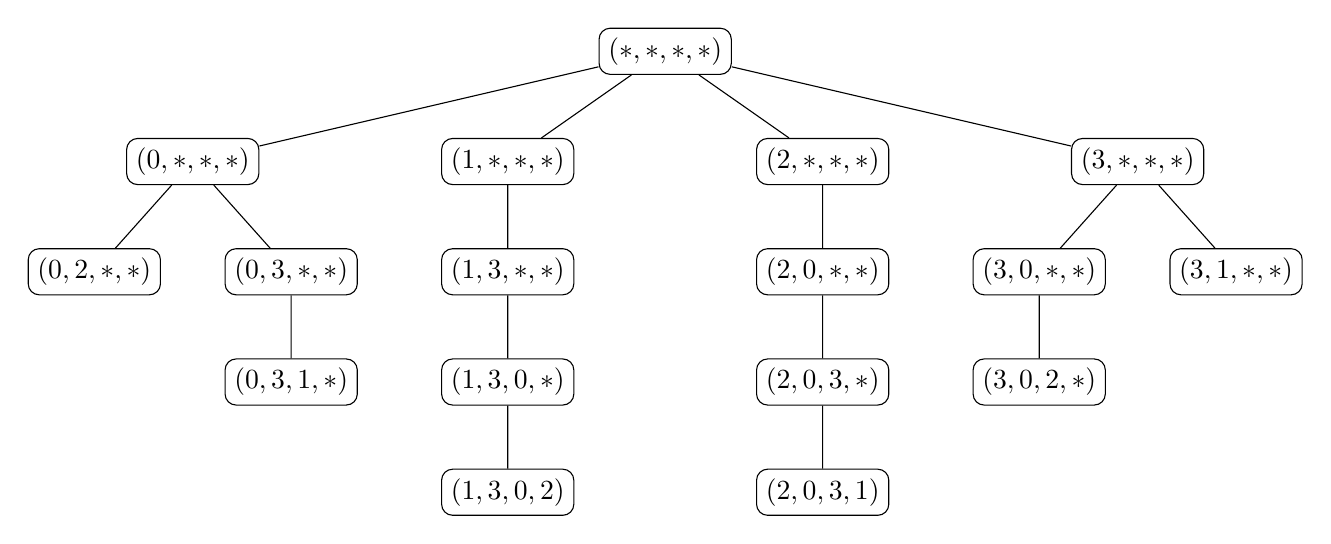
\begin{tikzpicture}[
  level 1/.style={sibling distance=40mm},
  level 2/.style={sibling distance=25mm},
  level 3/.style={sibling distance=18mm},
  level 4/.style={sibling distance=14mm},
  level distance=14mm,
  every node/.style={draw, rounded corners, align=center}
]

\node {$(\ast,\ast,\ast,\ast)$}
  child { node {$(0,\ast,\ast,\ast)$}
    child { node {$(0,2,\ast,\ast)$}
    }
    child { node {$(0,3,\ast,\ast)$}
      child { node {$(0,3,1,\ast)$}
      }
    }
  }
  child { node {$(1,\ast,\ast,\ast)$}
    child { node {$(1,3,\ast,\ast)$}
      child { node {$(1,3,0,\ast)$}
        child { node {$(1,3,0,2)$} }
      }
    }
  }
  child { node {$(2,\ast,\ast,\ast)$}
    child { node {$(2,0,\ast,\ast)$}
      child { node {$(2,0,3,\ast)$}
        child { node {$(2,0,3,1)$} }
      }
    }
  }
  child { node {$(3,\ast,\ast,\ast)$}
    child { node {$(3,0,\ast,\ast)$}
      child { node {$(3,0,2,\ast)$} }
    }
    child { node {$(3,1,\ast,\ast)$} }
  };

\end{tikzpicture}
\end{center}

\noindent\textbf{(3)代码:}
\begin{lstlisting}[language=C,style=codeStyle]
#include <iostream>
#include <math.h>
using namespace std;
int n = 8;      // 若做 4 皇后可改为 n=4
int total = 0;
int *c = new int[n];   // c[row] 表示第 row 行皇后所在列
bool is_ok(int row)
{
    for (int j = 0; j < row; j++)
    {
        // 同列:c[row] == c[j]
        // 同对角线:row + c[row] == j + c[j]
        // 同反对角线:row - c[row] == j - c[j]
        if (c[row] == c[j] ||
            row + c[row] == j + c[j] ||
            row - c[row] == j - c[j])
            return false;
    }
    return true;
}
void queen(int row)
{
    if (row == n)
        total++;
    else
    {
        for (int col = 0; col < n; col++)
        {
            c[row] = col;
            if (is_ok(row))
                queen(row + 1);
        }
    }
}
int main()
{
    queen(0);
    cout << total;
    return 0;
}
\end{lstlisting}

\noindent\textbf{(4)时间复杂度分析:}
设棋盘规模为 $n\times n$。
在回溯算法中,第 $row$ 行最多尝试 $n$ 个列位置,
每次尝试需要调用一次合法性检测函数 \texttt{is\_ok}。
该函数需要将当前皇后与之前已放置的 $row$ 个皇后进行比较,
其时间复杂度为 $O(row)$,最坏情况下为 $O(n)$。
在最坏情况下,回溯搜索树的结点数上界为
$n \cdot (n-1) \cdot (n-2) \cdots 1 = n!$
因此,算法的时间复杂度为$
T(n)=O(n\cdot n!)$

\noindent\textbf{空间复杂度分析:}
算法使用一个长度为 $n$ 的数组保存解向量,
同时递归调用的最大深度为 $n$,
因此空间复杂度为$S(n)=O(n).$

\noindent\textbf{2. 旅行售货员问题:}
某售货员要到若干城市去推销商品,已知各城市之间的路程(如下无向图所示)。
他要选定一条从驻地(城市 1)出发,经过每个城市一次,最后回到驻地的路线,使总的路程(或总旅行费)最小。
\begin{figure}[H]
  \centering
  \includegraphics[width=0.3\textwidth]{5-1-1.jpg}
\end{figure}

\begin{enumerate}
  \item [(1)]求解最优路线及其长度。
  \item [(2)]给出界限函数的设计以及求解过程中所采用的剪枝策略。
  \item [(3)]画出搜索空间树,标明发生剪枝的节点,以及树中的各个中间节点
        所对应的路径长度。
\end{enumerate}

\noindent\textbf{(1)最优解:}
最优路线为:$1 \rightarrow 3 \rightarrow 5 \rightarrow 4 \rightarrow 2 \rightarrow 1,$
其路径总长度为:16.

\noindent\textbf{(2)界限函数与剪枝策略:}

采用分支限界法求解。
设当前路径为部分路径 $P$,其已产生的路径长度为
$
\sum_{i=1}^{k-1} c(p_i,p_{i+1}),$

则其下界函数可设计为:
$
lb = \sum_{i=1}^{k-1} c(p_i,p_{i+1})
     + \sum_{v \in U} \frac{\min c(v)}{2},
$
其中 $U$ 为尚未访问的城市集合,
$\min c(v)$ 表示与城市 $v$ 相连的最小边权。
当某一结点的下界值不小于当前已知最优解时,则对该结点进行剪枝,不再继续扩展。

\noindent\textbf{(3)解空间树:}
\begin{figure}[htbp]
  \centering
  \includegraphics[width=0.9\textwidth]{5-1-2.jpg}
\end{figure}

\noindent\textbf{3.码头装箱问题:}
码头上有 $n$ 个集装箱要装上一艘载重量为 $C$ 的轮船,
其中集装箱 $i$ 的重量为 $w_i$,
请采用回溯法设计一个最优的装载方案,
即从全体集装箱中选取集装箱将该轮船尽可能地装满,
使得所装集装箱重量之和最接近 $C$。该问题等价于:
$$\max \sum_{i=1}^{n} w_i x_i$$
$$\text{s.t.}\ \sum_{i=1}^{n} w_i x_i \le C$$
$$x_i \in \{0,1\},\ 1 \le i \le n$$

\begin{enumerate}
  \item[(1)] 设集装箱的数量 $n=4$,
  轮船的载重量 $C=70$,
  每个集装箱的重量
  $W=\{30,50,20,10\}$,
  请给出本问题的解向量,
  并画出解空间树;
  \item[(2)] 给出搜索的剪枝策略;
  \item[(3)] 写出基于 C/C++ 的算法伪代码;
  \item[(4)] 分析所写算法的时间复杂性。
\end{enumerate}

\noindent\textbf{(1)解向量与解空间树:}

解向量定义为$
x=(x_1,x_2,\dots,x_n),$
其中
$
x_i=
\begin{cases}
1,& \text{选择装入第 } i \text{ 个集装箱};\\
0,& \text{不装入第 } i \text{ 个集装箱}.
\end{cases}
$

本题 $n=4, C=70, W=\{30,50,20,10\}$。

枚举可行装载中使总重量最大且不超过 $C$ 的方案:
$30+20+10=60,\quad 50+20=70,\quad 50+10=60,\quad 30+50=80(>70).$
其中最优为$50+20=70,$
对应解向量为$\boxed{x=(0,1,1,0)}.$

\begin{center}
\begin{forest}
for tree={
  draw, rounded corners, align=center,
  font=\scriptsize, inner sep=2pt,
  edge={-}, parent anchor=south, child anchor=north,
  l sep=10mm, s sep=12mm
}
[
  {(*,*,*,*)\\ cw=0}
  [
    {(1,*,*,*)\\ x1=1\\ cw=30}
    [
      {(1,1,*,*)\\ x2=1\\ cw=80}
      [{$\times$\\ OVER}, draw=none]
    ]
    [
      {(1,0,*,*)\\ x2=0\\ cw=30}
      [
        {(1,0,1,*)\\ x3=1\\ cw=50}
        [
          {(1,0,1,1)\\ x4=1\\ cw=60}
        ]
        [
          {(1,0,1,0)\\ x4=0\\ cw=50}
          [{$\times$\\ BOUND}, draw=none]
        ]
      ]
      [
        {(1,0,0,*)\\ x3=0\\ cw=30}
        [{$\times$\\ BOUND}, draw=none]
      ]
    ]
  ]
  [
    {(0,*,*,*)\\ x1=0\\ cw=0}
    [
      {(0,1,*,*)\\ x2=1\\ cw=50}
      [
        {(0,1,1,*)\\ x3=1\\ cw=70}
        [
          {(0,1,1,1)\\ x4=1\\ cw=80}
          [{$\times$\\ OVER}, draw=none]
        ]
        [
          {(0,1,1,0)\\ x4=0\\ cw=70},
          double
        ]
      ]
      [
        {(0,1,0,*)\\ x3=0\\ cw=50}
        [{$\times$\\ BOUND}, draw=none]
      ]
    ]
    [
      {(0,0,*,*)\\ x2=0\\ cw=0}
      [{$\times$\\ BOUND}, draw=none]
    ]
  ]
]
\end{forest}
\end{center}


\noindent\textbf{(2)搜索的剪枝策略:}
采用上界剪枝。设当前已装重量为 $cw$,当前最优可行解重量为 $bestw$,
剩余未处理集装箱重量之和为 $r$。
\begin{itemize}
  \item \textbf{约束剪枝:}若 $cw+w[i]>C$,则左子树(装入第 $i$ 个集装箱)不可行,直接剪去;
  \item \textbf{界限剪枝:}若 $cw+r\le bestw$,则即使把剩余所有集装箱都装入也不可能超过当前最优值,
        因此右子树(不装第 $i$ 个集装箱)可剪枝。
\end{itemize}

\noindent\textbf{(3)基于 C/C++ 的算法伪代码:}

\begin{lstlisting}[language=C,style=codeStyle]
void backtrack(int i)
{
    if (i > n) {            // 到达叶结点
        bestw = cw;         // 更新最优解
        return;
    }
    r -= w[i];              // 更新剩余重量
    if (cw + w[i] <= c) {   // 搜索左子树(装第 i 个)
        x[i] = 1;
        cw += w[i];
        backtrack(i + 1);
        cw -= w[i];
    }
    if (cw + r > bestw) {   // 搜索右子树(不装第 i 个)
        x[i] = 0;
        backtrack(i + 1);
    }
    r += w[i];              // 回退到上一层
}
\end{lstlisting}

\noindent\textbf{(4)时间复杂性分析:}
最坏情况下,回溯需要遍历所有解空间结点,
每个集装箱都有“装/不装”两种选择,因此结点数为 $2^n$ 量级。
剪枝只能减少实际搜索量,但不改变最坏情况上界。

因此该算法最坏时间复杂度为:$\boxed{O(2^n)}.$
递归深度为 $n$,并使用长度为 $n$ 的数组保存解向量,
空间复杂度为:$\boxed{O(n)}.$

\noindent\textbf{4.旅行商问题(TSP):}针对旅行商 TSP 问题,
\begin{enumerate}
  \item[(1)]采用 C/C++/Java/Python 语言伪代码,
  写出采用回溯法求解该问题的递归或非递归算法,
  同时:
  \begin{enumerate}
    \item[(i)] 设计采用的界限函数;
    \item[(ii)] 说明回溯过程中对结点采用的剪枝策略。
  \end{enumerate}
  \item[(2)] 针对下面无向图,
  以结点 1 为起始城市,
  用上述算法求解:
  \begin{enumerate}
    \item[(i)] 一条最短回路及其长度;
    \item[(ii)] 画出回溯搜索过程中生成的解空间树,
    说明发生剪枝的结点,
    以及树中各个叶结点、非叶结点对应的路径长度。
  \end{enumerate}
\end{enumerate}

\begin{figure}[H]
  \centering
  \includegraphics[width=0.3\textwidth]{5-2.png}
\end{figure}

\noindent\textbf{解答:}
\noindent\textbf{(1)回溯算法伪代码、界限函数与剪枝策略:}

\noindent\textbf{(1-i)界限函数:}
设当前已确定的部分路径为
$1=x_1 \rightarrow x_2 \rightarrow \cdots \rightarrow x_{i-1},$
其当前路径长度为 $cc$。
则对任一候选扩展 $x_i=x_j$(从未访问集合中选)时,
\textbf{下界(界限函数)}可取为$LB = cc + a[x_{i-1}][x_j].$
因为后续还要继续走若干边,总代价一定不小于已发生的代价(加上当前准备走的这一步)。

\noindent\textbf{(1-ii)剪枝策略:}
设当前已知最优回路长度为 $bestc$。
当扩展到候选结点 $x_j$ 时,若
$cc + a[x_{i-1}][x_j] \ge bestc,$
则即使继续向下搜索也不可能得到更优解,因此剪枝,不再递归该分支。

\noindent\textbf{伪代码:}
\begin{lstlisting}[language=C++,style=codeStyle]
template<class Type>
void Traveling<Type>::Backtrack(int i)
{
    if (i == n) {
        if (a[x[n-1]][x[n]] != NoEdge &&
            a[x[n]][x[1]] != NoEdge &&
            (cc + a[x[n-1]][x[n]] + a[x[n]][x[1]] < bestc
             || bestc == NoEdge)) {
            bestc = cc + a[x[n-1]][x[n]] + a[x[n]][x[1]];
        }
    }
    else
        for (int j = i; j <= n; j++) {
            if (a[x[i-1]][x[j]] != NoEdge &&
                (cc + a[x[i-1]][x[j]] < bestc
                 || bestc == NoEdge)) {
                swap(x[i], x[j]);
                cc += a[x[i-1]][x[i]];
                Backtrack(i + 1);
                cc -= a[x[i-1]][x[i]];
                swap(x[i], x[j]);
            }
        }
}
\end{lstlisting}

\noindent\textbf{(2)对给定无向图(起点为 1)的求解结果:}

图中边权为:
$a_{12}=10,\ a_{13}=20,\ a_{14}=5,\ a_{23}=15,\ a_{24}=5,\ a_{34}=5.$

\noindent\textbf{(2-i)一条最短回路及其长度:}

枚举(或按回溯搜索)可得最短回路长度为
$\boxed{35}.$
例如一条最短回路为:
$
\boxed{1 \rightarrow 2 \rightarrow 3 \rightarrow 4 \rightarrow 1},
$
其长度:
$10+15+5+5 = 35.$
(其逆序回路 $1\rightarrow 4\rightarrow 3\rightarrow 2\rightarrow 1$ 也同样为 35。)

\noindent\textbf{(2-ii)回溯搜索生成的解空间树(含剪枝结点与路径长度):}

以下树按代码的搜索顺序(从小下标到大下标)展开。
结点标注“当前部分路径 / 当前累计长度 $cc$”;叶子结点标注“回路总长度”;
被剪枝分支用 $\times$ 标出(条件为 $cc+\text{下一条边}\ge bestc$ 或超越当前最优)。

\begin{center}
\begin{forest}
for tree={
  draw,
  rounded corners,
  align=center,
  font=\scriptsize,
  inner sep=2pt,
  edge={-},
  parent anchor=south,
  child anchor=north,
  l sep=10mm,
  s sep=12mm
}
[
  {start: (1)\\ cc=0}
  [
    {(1,2)\\ cc=10}
    [
      {leaf: (1,2,3,4,1)\\ total=35},
      double
    ]
    [
      {leaf: (1,2,4,3,1)\\ total=40}
    ]
  ]
  [
    {(1,3)\\ cc=20}
    [
      {$\times$\\ prune\\ (1,3,2,*)\\ cc would be 35},
      draw=none
    ]
    [
      {leaf: (1,3,4,2,1)\\ total=40}
    ]
  ]
  [
    {(1,4)\\ cc=5}
    [
      {leaf: (1,4,3,2,1)\\ total=35}
    ]
    [
      {leaf: (1,4,2,3,1)\\ total=45}
    ]
  ]
]
\end{forest}
\end{center}


